%Autor: Simon Walker
%Version: 1.0
%Datum: 30.11.2019
%Lizenz: CC BY-NC-SA

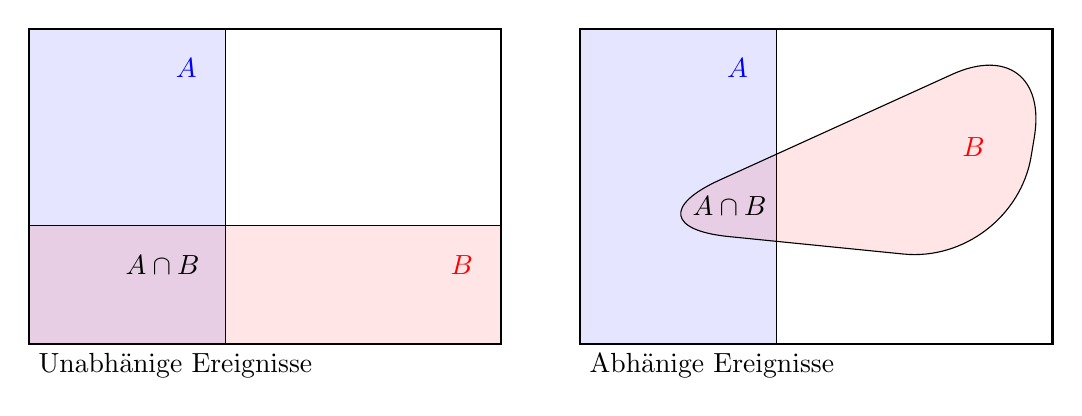
\begin{tikzpicture}

%	\newcommand{\HelpCords}[4]{
%		\draw [help lines] (#1,#2) grid (#3,#4);
%		\foreach \i in {#1,..., #3}
%		\node [below] at (\i,#2) {$\i$};
%		\foreach \i in {#2,..., #4}
%		\node [left] at (#1,\i) {$\i$};
%	}

	\filldraw [draw=black, fill=blue, fill opacity=.1] (0,0) rectangle (2.5,4);
	\filldraw [draw=black, fill=red, fill opacity=.1] (0,0) rectangle (6,1.5);
	\draw [thick] (0,0) rectangle (6,4);
	\node[blue] at (2, 3.5) {$A$};
	\node[red] at (5.5, 1) {$B$};
	\node at (1.7, 1) {$A\cap B$};
	\node[below right] at (0,0) {Unabhänige Ereignisse};
	
	
	\filldraw [draw=black, fill=blue, fill opacity=.1] 
	(7,0) rectangle (9.5,4);
	\filldraw [draw=black, fill=red, fill opacity=.1, rounded corners=14mm, smooth] 
	(13,4) -- (7.5, 1.5) -- (12.5, 1) -- cycle;
	\draw [thick] (7,0) rectangle (13,4);
	\node[blue] at (9, 3.5) {$A$};
	\node[red] at (12, 2.5) {$B$};
	\node at (8.9, 1.75) {$A\cap B$};
	\node[below right] at (7,0) {Abhänige Ereignisse};
	
%	\HelpCords{0}{0}{6}{4}
%	\HelpCords{7}{0}{13}{4}
	
	
\end{tikzpicture}